\documentclass[12pt,letterpaper]{article}
\usepackage[utf8]{inputenc}
\usepackage[english]{babel}
\usepackage{fullpage}
\usepackage[top=2cm, bottom=4.5cm, left=2.5cm, right=2.5cm]{geometry}
\usepackage{amsmath,amsthm,amsfonts,amssymb,amscd}
\usepackage{lastpage}
\usepackage{enumerate}
\usepackage{fancyhdr}
\usepackage{mathrsfs}
\usepackage{xcolor}
\usepackage{graphicx}
\usepackage{listings}
\usepackage{hyperref}

\hypersetup{%
  colorlinks=true,
  linkcolor=blue,
  linkbordercolor={0 0 1}
}

\renewcommand\lstlistingname{Algorithm}
\renewcommand\lstlistlistingname{Algorithms}
\def\lstlistingautorefname{Alg.}


\setlength{\parindent}{0.0in}
\setlength{\parskip}{0.05in}

% Edit these as appropriate
\newcommand\course{Algorithms II}
\newcommand\hwnumber{2}                  % <-- homework number
\newcommand\NetIDa{17CS10056}           % <-- NetID of person #1
\newcommand\NetIDb{Ayush Tiwari}           % <-- NetID of person #2 (Comment this line out for problem sets)

\pagestyle{fancyplain}
\headheight 35pt
\lhead{\NetIDa}
\lhead{\NetIDa\\\NetIDb}                 % <-- Comment this line out for problem sets (make sure you are person #1)
\chead{\textbf{\Large Tutorial \hwnumber}}
\rhead{\course \\ \today}
\lfoot{}
\cfoot{}
\rfoot{\small\thepage}
\headsep 1.5em

\begin{document}

\section*{Problem Statement}
    $P[1..m]$ is an input list of n points on $xy$-plane. Assume that all n points have distinct $x$-coordinates and distinct $y$-coordinates. Let $p\textsubscript{L}$ and $p\textsubscript{R}$ denote the leftmost and points of $P$, respectively. The task is to find the polygon $Q$ with $P$ as its vertex set such that the following conditions are satisfied.

    \begin{enumerate}
        \item The upper vertex chain of $Q$ is $x$-monotone (increasing) from $p\textsubscript{L}$ to $p\textsubscript{R}$.
        \item The lower vertex chain of $Q$ is $x$-monotone (decreasing) from $p\textsubscript{R}$ to $p\textsubscript{L}$.
        \item Perimeter of $Q$ is minimum.
    \end{enumerate}

\section*{Algorithm}

    Say the $n$ points are $x\textsubscript{1}, x\textsubscript{2},..., x\textsubscript{n}$. Let's assume them to be ordered by their $x$-coordinates i.e. $x\textsubscript{1}$ is the leftmost and $x\textsubscript{n}$ is the rightmost.

    \begin{figure}[htp]
    \centering
        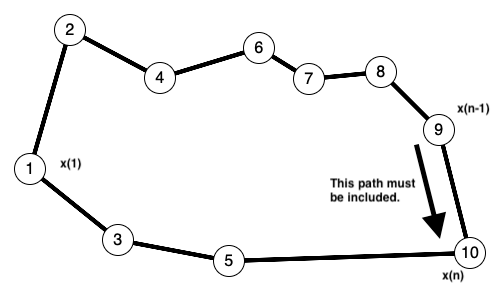
\includegraphics[width=8cm]{TOCFctRDSbmtFSit5.png}
            \caption{Path $(x\textsubscript{n-1}, x\textsubscript{n})$}
        \label{fig:galaxy}
    \end{figure}

    \newtheorem{lemma}{Lemma}
    \begin{lemma}
        The segment $(x\textsubscript{n-1}, x\textsubscript{n})$ will be contained in the polygon $Q$.
    \end{lemma}

    \begin{proof}
        Suppose the segment $(x\textsubscript{n-1}, x\textsubscript{n})$ is not contained in $Q$. This means that the polygon must have a portion like this - $x\textsubscript{i}..x\textsubscript{n-1}..x\textsubscript{j}..x\textsubscript{n}$. However we know that both $x\textsubscript{i}$ and $x\textsubscript{j}$ have smaller coordinates than $x\textsubscript{n-1}$ which means that the portion is not $x$-monotone, which is a contradiction.
    \end{proof}

    Now let's frame this problem as finding a path from $x\textsubscript{n}$ back to itself such that the initially we strictly travel left to $x\textsubscript{1}$ and then we strictly travel right to $x\textsubscript{n}$. One possible question that might arise is - \textbf{Why should we expect the path to be non-crisscrossing?}. We will answer this later. For now assume that the result is a normal polygon.\\\\
    From lemma 1, it suffices to find the length of the minimal path going from $x\textsubscript{n}$ strictly to the left upto $x\textsubscript{1}$ - leaving out $x\textsubscript{n-1}$ - and then from $x\textsubscript{1}$ strictly to the right upto $x\textsubscript{n-1}$ and add it to the distance between $x\textsubscript{n}$ and $x\textsubscript{n-1}$. \\

    We now make the following observations :

    \begin{enumerate}
        \item Any acceptable path from $x\textsubscript{n}$ to $x\textsubscript{n-1}$ must start with a first edge $(x\textsubscript{n}, x\textsubscript{k})$ for some $k < n-1$.
        \item Since we must visit all points, and since from $x\textsubscript{k}$ we can only continue to the left, all the points $x\textsubscript{k+1}, x\textsubscript{k+2}, ... , x\textsubscript{n-1}$ must necessarily be visited on the way from left to right (and in this order). So, necessarily our path ends with $x\textsubscript{k+1}\longrightarrow x\textsubscript{k+2}\longrightarrow ... \longrightarrow x\textsubscript{n-1}$.
    \end{enumerate}

    \begin{figure}[htp]
    \centering
        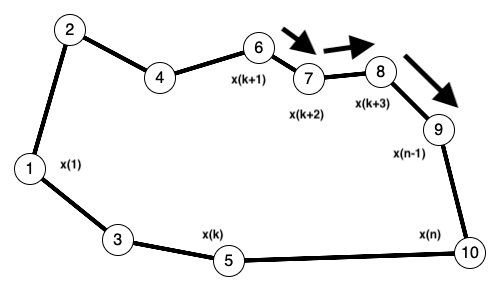
\includegraphics[width=8cm]{TOCFctRDSbmtFSit.png}
            \caption{These paths must be visited on the return journey.}
        \label{fig:galaxy}
    \end{figure}

    So far we have figured out that an acceptable path from $x\textsubscript{n}$ to $x\textsubscript{n-1}$ has the form
    \begin{center}
        $x\textsubscript{n} \longrightarrow  x\textsubscript{k} \longrightarrow \enspace ??? \longrightarrow  x\textsubscript{k+1} \longrightarrow  x\textsubscript{k+2} \longrightarrow  ... \longrightarrow  x\textsubscript{n-1}$.
    \end{center}

    where $\longrightarrow  x\textsubscript{k} \longrightarrow \enspace ??? \longrightarrow  x\textsubscript{k+1}$ is in itself an acceptable path (satisfying all the constraints) from $x\textsubscript{k}$ to $x\textsubscript{k+1}$ with $k < n-1$. \\

    If we want to minimize the length of path from $x\textsubscript{n}$ to $x\textsubscript{n-1}$, we must also minimize the length of the path from $x\textsubscript{k}$ to $x\textsubscript{k+1}$ (which is the same as the length of the acceptable path from $x\textsubscript{k+1}$ to $x\textsubscript{k}$).

    For any $i > 1$ let $l(i)$ denote the length of the acceptable minimum length path from $x\textsubscript{i}$ to $x\textsubscript{i-1}$. The preceeding arguments imply that :

    \begin{center}
        $l(n) = d(x\textsubscript{n}, x\textsubscript{k}) + l(k+1) + \sum_{m=k+1}^{n-2} d(x\textsubscript{m}, x\textsubscript{m+1})$
    \end{center}

    \begin{figure}[htp]
    \centering
        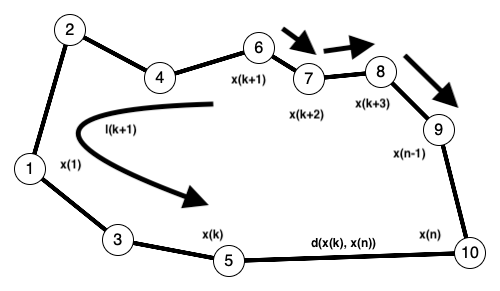
\includegraphics[width=8cm]{TOCFctRDSbmtFSit62.png}

        \label{fig:galaxy}
    \end{figure}

    For some $k < n$ we have :

    \begin{center}
        $l(n) = \min_{1<i<n} \big{[}\enspace d(x\textsubscript{n}, x\textsubscript{i-1}) + l(i) + \sum_{m=k+1}^{n-2} d(x\textsubscript{m}, x\textsubscript{m+1})\enspace  \big{]}$
    \end{center}

    The exact same reasoning also applies on such paths for any $2 < p < n$ i.e we have obtained the recursion :

    \begin{center}
        $l(p) = \min_{1<i<p} \big{[}\enspace d(x\textsubscript{p}, x\textsubscript{i-1}) + l(i) + \sum_{m=k+1}^{p-2} d(x\textsubscript{m}, x\textsubscript{m+1})\enspace  \big{]}$
    \end{center}

    And $l(2) = d(x\textsubscript{2}, x\textsubscript{1})$. We can use this recursion to successively calculate $l(p)$ for $p=2,...,n$, then the required lenght for all sets of points would be :

    \begin{center}
        $l(n) + d(x\textsubscript{n}, x\textsubscript{n-1})$
    \end{center}

    \subsection*{How to construct he path?}

        To construct the optimal path satisfying the constraint we only need to store the value of $i$ that optimizes $l(p)$ for all values of $p$. From this we can find the neighbour of $x\textsubscript{n}$ and then the neighbour of that neighbour and so on.

    \subsection*{Why would the resulting path be a polygon?}
        Now coming back to the assumption. It is actually very easy to see that for any path that consists of criss crossing edges we can construct a shorter path without having crossing edges. This is a direct consequence of the triangle inequality.

        \begin{figure}[htp]
            \centering
                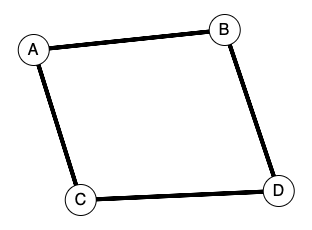
\includegraphics[width=5cm]{aPsbRwcprpkjDGQy.png}
                \caption{Polygon 1}
            \label{fig:galaxy}
        \end{figure}

        Consider an example where the paths $AB$ and $CD$ in the above polygon are replaced by $AD$ and $BC$. Also, note that $Q$ is the intersection $AD$ and $BC$ in the new polygon.

        \begin{figure}[htp]
            \centering
                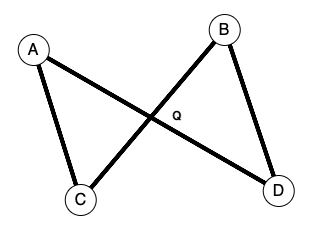
\includegraphics[width=5cm]{JuCfnLBJBYpfEIdK.png}
                \caption{Polygon 2}
            \label{fig:galaxy}
        \end{figure}

        By triangle inequlity $BQ + AQ$ in the second polygon must be greater than $AB$ in the first polygon. \\
        Also, $CQ + DQ$ in the second polygon must be grater than $CD$ in the first polygon. \\
        The first polygon must have smaller total path length than the second polygon. \\

        \emph{Therefore, we can say that the result of the algorithm will always be a polygon.}

\section*{Time and Space Complexities}

    \begin{enumerate}
        \item The time complexity is $\mathcal{O}(n^2)$.\\\\
        \underline{Justification} -
            It can be seen that for each value of $p > 2$ we have to take the minimum of $p-2$ terms. Also, note that the value of $\sum_{m=k+1}^{p-2} d(x\textsubscript{m}, x\textsubscript{m+1})$ can be calculated in $\mathcal{O}(1)$ time after a pre-processing that takes $\mathcal{O}(n^2)$ time. Therefore the required time complexity calculate will take the form $\sum_i (i-2)$ which will lead to a an overall time complexity of $\mathcal{O}(n^2)$.

        \item The space complexity is also $\mathcal{O}(n)$.

        \underline{Justification} -
            As explained in the previous section, we need to store the value of $i$ that optimizes $l(p)$ for all values of $p$, where $2 < p < n$. Therefore, we require $\mathcal{O}(n)$ space.

    \end{enumerate}

\end{document}
